\documentclass[tikz,border=8pt]{standalone}
% Shared UMM figure style (journal-consistent palette + line weights)
\usepackage{tikz}
\usepackage{pgfplots}
\pgfplotsset{compat=1.18}
\usetikzlibrary{arrows.meta,calc,positioning,decorations.pathmorphing,patterns,shapes.geometric,fit,backgrounds}
% Palette: grayscale + single accent (deep teal)
\definecolor{ummAccent}{HTML}{0B6E6E}
\definecolor{ummAccentLight}{HTML}{4A9B9B}
\definecolor{ummDark}{HTML}{1A1A1A}
\definecolor{ummGray}{HTML}{555555}
\definecolor{ummLightGray}{HTML}{AAAAAA}
\definecolor{ummFill}{HTML}{E8F2F2}
\definecolor{ummGas}{HTML}{C45C26}
\definecolor{ummGasLight}{HTML}{F0C4A8}
\definecolor{ummGalaxy}{HTML}{2C3E50}
\definecolor{ummLens}{HTML}{0B6E6E}
\pgfplotsset{
  umm axis/.style={
    axis lines=left,
    axis line style={ummDark, line width=0.8pt},
    tick style={ummDark, line width=0.6pt},
    tick label style={font=\footnotesize, ummDark},
    label style={font=\small, ummDark},
    title style={font=\small\bfseries, ummDark},
    grid=both,
    major grid style={ummLightGray, opacity=0.35, line width=0.3pt},
    minor grid style={ummLightGray, opacity=0.15, line width=0.2pt},
    every axis plot/.append style={line width=1.3pt},
    legend style={font=\footnotesize, draw=ummLightGray, fill=white, fill opacity=0.92, text opacity=1},
    clip=false,
  },
}
\newcommand{\ummLineW}{1.25pt}
\newcommand{\ummLineWthin}{0.9pt}
\tikzset{
  umm arr/.style={-{Latex[length=2.2mm,width=1.6mm]}},
}

\begin{document}
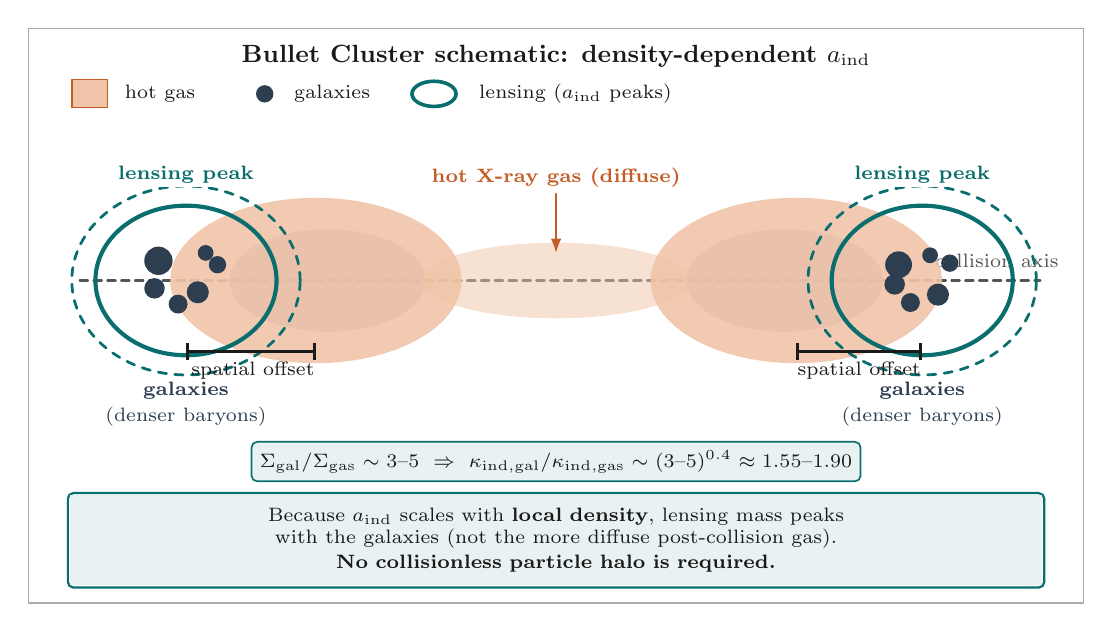
\begin{tikzpicture}[font=\small, line cap=round, line join=round]
  % Frame
  \draw[ummLightGray, line width=0.6pt] (-0.15,-1.75) rectangle (13.25,5.55);
  \node[font=\bfseries\small, ummDark] at (6.55,5.2)
    {Bullet Cluster schematic: density-dependent $a_{\mathrm{ind}}$};

  % Legend at top
  \fill[ummGasLight] (0.4,4.55) rectangle (0.85,4.9);
  \draw[ummGas, line width=0.5pt] (0.4,4.55) rectangle (0.85,4.9);
  \node[font=\scriptsize, anchor=west, ummDark] at (0.95,4.72) {hot gas};
  \fill[ummGalaxy] (2.85,4.72) circle (0.11);
  \node[font=\scriptsize, anchor=west, ummDark] at (3.1,4.72) {galaxies};
  \draw[ummLens, line width=1.3pt] (5.0,4.72) ellipse (0.28 and 0.16);
  \node[font=\scriptsize, anchor=west, ummDark] at (5.45,4.72) {lensing ($a_{\mathrm{ind}}$ peaks)};

  % Collision axis
  \draw[ummGray, densely dashed, line width=0.8pt] (0.5,2.35) -- (12.7,2.35);
  \node[font=\scriptsize, ummGray] at (12.15,2.6) {collision axis};

  % ---- Diffuse hot gas (offset inward from galaxies) ----
  \fill[ummGasLight, opacity=0.9]
    (3.5,2.35) ellipse (1.85 and 1.05);
  \fill[ummGas!40, opacity=0.7]
    (3.65,2.35) ellipse (1.25 and 0.65);
  \fill[ummGasLight, opacity=0.9]
    (9.6,2.35) ellipse (1.85 and 1.05);
  \fill[ummGas!40, opacity=0.7]
    (9.45,2.35) ellipse (1.25 and 0.65);
  \fill[ummGasLight, opacity=0.5]
    (6.55,2.35) ellipse (1.7 and 0.48);

  \node[font=\scriptsize\bfseries, ummGas] at (6.55,3.65) {hot X-ray gas (diffuse)};
  \draw[ummGas, line width=0.7pt, -{Latex[length=1.8mm]}]
    (6.55,3.45) -- (6.55,2.7);

  % ---- Galaxies ----
  \foreach \dx/\dy/\s in {-0.35/0.25/0.18, 0.15/-0.15/0.14, 0.4/0.2/0.11,
                          -0.1/-0.3/0.12, 0.25/0.35/0.1, -0.4/-0.1/0.13} {
    \fill[ummGalaxy] (1.85+\dx, 2.35+\dy) circle (\s);
  }
  \node[font=\scriptsize\bfseries, ummGalaxy] at (1.85,0.95) {galaxies};
  \node[font=\scriptsize, ummGalaxy] at (1.85,0.62) {(denser baryons)};

  \foreach \dx/\dy/\s in {-0.3/0.2/0.17, 0.2/-0.18/0.14, 0.35/0.22/0.11,
                          -0.15/-0.28/0.12, 0.1/0.32/0.1, -0.35/-0.05/0.13} {
    \fill[ummGalaxy] (11.2+\dx, 2.35+\dy) circle (\s);
  }
  \node[font=\scriptsize\bfseries, ummGalaxy] at (11.2,0.95) {galaxies};
  \node[font=\scriptsize, ummGalaxy] at (11.2,0.62) {(denser baryons)};

  % ---- Lensing peaks with galaxies ----
  \draw[ummLens, line width=1.5pt]
    (1.85,2.35) ellipse (1.15 and 0.95);
  \draw[ummLens, line width=1.0pt, dashed]
    (1.85,2.35) ellipse (1.45 and 1.2);
  \node[font=\scriptsize\bfseries, ummLens, fill=white, inner sep=1.5pt]
    at (1.85,3.7) {lensing peak};

  \draw[ummLens, line width=1.5pt]
    (11.2,2.35) ellipse (1.15 and 0.95);
  \draw[ummLens, line width=1.0pt, dashed]
    (11.2,2.35) ellipse (1.45 and 1.2);
  \node[font=\scriptsize\bfseries, ummLens, fill=white, inner sep=1.5pt]
    at (11.2,3.7) {lensing peak};

  % Offset bars: galaxy center to gas center
  \draw[ummDark, line width=1.0pt, {|[width=2.2mm]}-{|[width=2.2mm]}]
    (1.85,1.45) -- (3.5,1.45);
  \node[font=\scriptsize, ummDark] at (2.7,1.2) {spatial offset};

  \draw[ummDark, line width=1.0pt, {|[width=2.2mm]}-{|[width=2.2mm]}]
    (9.6,1.45) -- (11.2,1.45);
  \node[font=\scriptsize, ummDark] at (10.4,1.2) {spatial offset};

  % Quantitative contrast annotation
  \node[font=\scriptsize, ummDark, align=center,
        draw=ummAccent, line width=0.6pt, rounded corners=2pt,
        fill=ummFill, inner sep=3pt]
    at (6.55,0.05)
    {$\Sigma_{\mathrm{gal}}/\Sigma_{\mathrm{gas}}\sim 3$--$5$
     $\;\Rightarrow\;$
     $\kappa_{\mathrm{ind,gal}}/\kappa_{\mathrm{ind,gas}}\sim(3$--$5)^{0.4}\approx 1.55$--$1.90$};

  % Bottom key message (fully inside box)
  \draw[ummAccent, line width=0.8pt, rounded corners=2pt]
    (0.35,-1.55) rectangle (12.75,-0.35);
  \fill[ummFill] (0.38,-1.52) rectangle (12.72,-0.38);
  \node[font=\scriptsize, ummDark, align=center, text width=12.0cm] at (6.55,-0.95)
    {Because $a_{\mathrm{ind}}$ scales with \textbf{local density}, lensing mass peaks with the galaxies
     (not the more diffuse post-collision gas).\\[0.15em]
     \textbf{No collisionless particle halo is required.}};
\end{tikzpicture}
\end{document}
